\chapter{Compiler}
\label{chap:Compiler}

Programmiersprachen dienen als Verständigungsmittel zwischen Programmierern und Rechenanlagen wie z.B Smartphones.  Diese Sprachen haben sich in der Vergangenheit dabei immer mehr an die  Terminologie eines bestimmtes Anwendungsgebietes angenähert. Durch diese Entwicklung eigneten sich Programmiersprachen direkt für die Dokumentation von entwickelten Algorithmen und Anwendungen, entfernten sich jedoch weiter von den Gegebenheiten des realen Rechners.\footcite[Vgl.][S. 15]{Schneider1975} Die Beziehung zwischen Softwareentwicklern und Rechenanlagen mit Hilfe von Programmiersprachen wird in Abbildung \ref{fig:Programmiersprachen als Schnittstelle} dargestellt. 

\begin{figure}[!ht]
 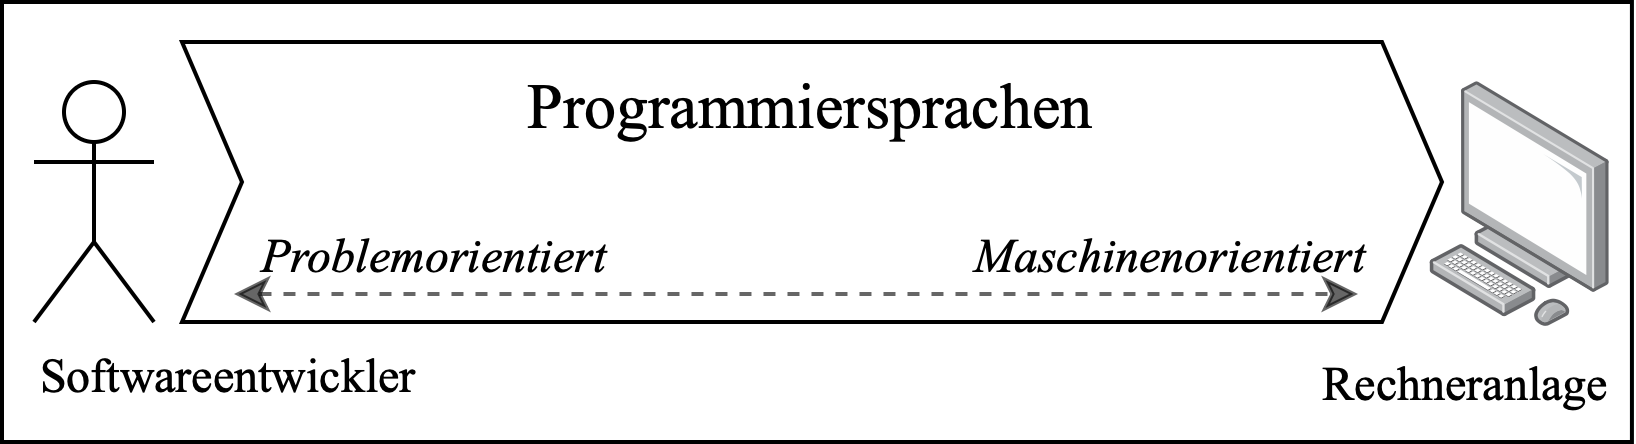
\includegraphics[width=\textwidth,height=\textheight,keepaspectratio]{Images/LanguageIntermediary.png}
 \caption{Programmiersprachen als Schnittstelle}
 \label{fig:Programmiersprachen als Schnittstelle}
\end{figure}

Für die Ausführung einer in einer problemorientierten Programmiersprache geschriebenen Anwendung ist es notwendig, die Sprache in eine maschinenorientierte Form zu überführen. \footcite[Vgl.][S. 15]{Schneider1975} Bereits im Jahre 1952 stelle Rutishauser fest,  dass Computer in der Lage sind,  diesen Übersetzungsvorgang selbst durchzuführen.\footcite[Vgl.][S. 312]{Rutishauser1952} 
Durch die Möglichkeit zur automatischen Übersetzung von problemorientierten Programmiersprachen konnten Hochsprachen entwickelt werden, die menschenfreundliche Sprachelemente anstatt Maschineninstruktionen verwenden. \footcite[Vgl.][S. 47]{Wagenknecht2014}
\section{ Grundbegriffe}
Diese historische Einführung zeigt,  dass Software zur automatisierten Übersetzung schon seit der Mitte des letzten Jahrhunderts thematisiert wurde, so hat sich in der Wissenschaft eine einheitliche Definition ergeben.  \citeauthor{Ullmann2008} beschreibt die sogenannten Compiler im Jahre \citeyear{Ullmann2008} wie folgt:\footcite[Vgl.][S. 1]{Ullmann2008} 
\begin{Def}[Compiler]
Ein Compiler ist ein Programm, welches ein anderes Programm aus einer Quellsprache in ein gleichwertiges Programm einer Zielsprache übersetzen kann.
\end{Def} 
\vspace{-1em}

Aus der Definition lässt sich ein für diese Arbeit relevanter Fakt ableiten: Compiler sind nicht ausschließlich Übersetzer zwischen problemorientierten und maschinenorientierten Programmiersprachen.  Sie sind ausschließlich für die Übersetzung von einer Quellsprache in eine Zielsprache verantwortlich.  Auch wenn der Begriff Programm für jedermann geläufig ist,  kann es  passieren,  dass von verschiedenen Repräsentationen gesprochen wird.  So können alle drei der folgenden Begriffe als Programm bezeichnet werden: Der Quelltext,  das ausführbare Programm und der laufende Prozess auf einem Computer.  Für das weitere Verständnis dieser Arbeit ist mit dem Begriff Programm die ausführbare Anwendung auf den Smartphones des Anwenders gemeint.  

Neben der Übersetzung von problem- zu maschinenorientierter Sprache gibt es ebenfalls Compiler, die andere Ziele verfolgen. Dazu gehören zum Beispiel die sogenannten Binärübersetzer,  die den Binärcode eines Programmes für andere Rechner überführen,  sodass er auf diesen ausgeführt werden kann.  \footcite[Vgl.][S. 27]{Ullmann2008} Ein
Source-to-Source Compiler,  häufig auch als \glqq Transpiler\grqq{} bezeichnet,  ist ebenfalls eine besondere Ausprägung eines Compilers, die sich wie folgt definieren lässt.  \footcite[Vgl.][S. 1629]{IJCSIT2015}
\begin{Def}[Source-to-Source Compiler]
Ein Source-to-Source-Compiler ist ein Compiler, bei dem sowohl die Quellsprache als auch die Zielsprache eine Hochsprache ist.
\end{Def}
\vspace{-1em}

Der Begriff Hochsprache ist dabei ein Synonym für die bereits eingeführten problemnahen Sprachen wie zum Beispiel C++,  Java,  \Csharp{} oder Dart,  die für den Menschen les- und änderbar sind. \footcite[Vgl.][S. 9]{Eisenecker2008} 

\section{Compiler Struktur}
Zur Übersetzung von Programmen bearbeiten Compiler zwei Teilaufgaben,  die Analyse und die Synthese. Während der Analyse wird das Programm in seine Bestandteile zerlegt und mit einer grammatikalischen Struktur versehen. Diese wird anschließend verwendet, um eine Zwischendarstellung zu generieren.  Dabei wird überprüft, ob das Programm syntaktisch und semantisch fehlerfrei ist oder ob der Programmierer Änderungen vornehmen muss. \footcite[Vgl.][S. 6f]{Ullmann2008} Die Syntax bezeichnet den Aufbau eines Programms,  sie legt fest wie Sprachelemente aus anderen Sprachelementen zusammengesetzt sind.  Im Gegensatz dazu beschreibt die Semantik die Bedeutung der Sprachelemente. \footcite[Vgl.][S. 36]{Schneider1975}  Außerdem werden bei der Analyse Informationen über das Quellprogramm gesammelt und in der sogenannten Symboltabelle abgelegt.  Die Synthese konstruiert aus der Zwischendarstellung und den Informationen aus der Symboltabelle das gewünschte Zielprogramm.  Der Teil des Compilers, der sich mit der Analyse befasst wird oft als Front-End bezeichnet, derjenige der für die Synthese zuständig ist als Back-End.  \footcite[Vgl.][S. 6f]{Ullmann2008}

Der Vorgang des Kompilierens lässt sich basierend auf diesen zwei Teilaufgaben nach \citeauthor{Ullmann2008} in mehrere Phasen unterteilen,  die in Abbildung \ref{fig:Compilerphasen} grafisch dargestellt sind und in diesem Abschnitt detailliert beschrieben werden.  \footcite[Vgl.][S. 6]{Ullmann2008}

\begin{figure}[!ht]
 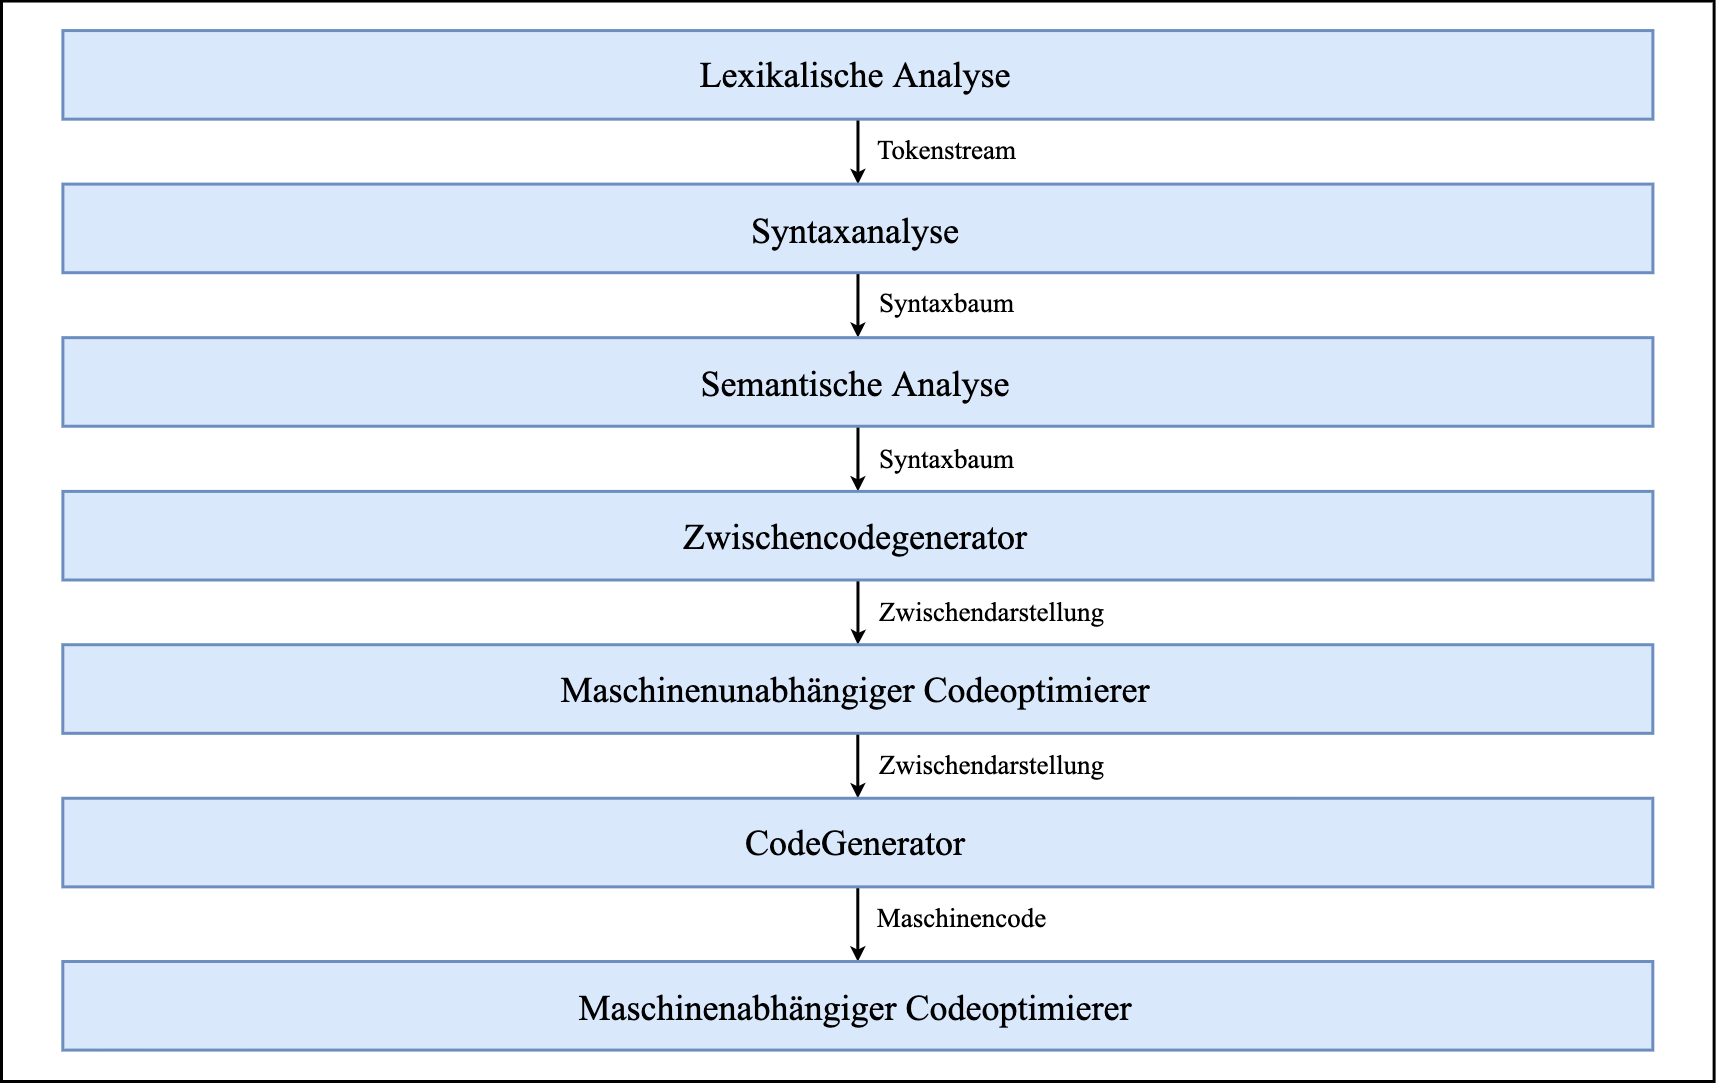
\includegraphics[width=\textwidth,keepaspectratio]{Images/Compiler/Phasen.png}
 \caption[Phasen der Kompilierung]{Phasen der Kompilierung\protect\footcite{Ullmann2008}}
 \label{fig:Compilerphasen}
\end{figure}
\footnotetext{Abbildung in Anlehnung an Ullman et al. 2008, S.6.}


\section{Lexikalische Analyse}
Die erste Phase eines Compilers ist die lexikalische Analyse,  die den Quelltext in Lexeme untergliedert.  Ein Lexem ist die Folge von Zeichen im Quellprogramm,  die als Instanz eines Tokens erkannt wurden.  Dabei ist ein Token ein Paar aus Namen und einem optionalen Attributwert,  wobei der Name zum Beispiel ein bestimmtes Schlüsselwort, oder eine Folge von Eingabezeichen sein kann und der Attributwert auf einen Eintrag in der Symboltabelle verweist.  \footcite[Vgl.][S. 135 f.]{Ullmann2008} In Tabelle \ref{tab:Tokens} werden einige beispielhafte Tokens aufgeführt sowie die Information darüber, aus welchen Lexemen diese extrahiert werden.

\begin{table}[!ht]
\begin{tabularx}{\textwidth}{|l|X|l|}
\hline

   \textbf{Token} & \textbf{Beschreibung} & \textbf{Lexem} \\
\hline
if             & Zeichen i,f           & if                      \\ 
comparison     & Vergleichsoperatoren  & \textless{}=            \\ 
id             & Buchstaben            & pi                      \\ 
number         & Numerische Konstanten    & 3.14159               \\    
\hline

\end{tabularx}
\caption[Token-Beispiele]{Token-Beispiele \protect\footcite{Ullmann2008}}
 \label{tab:Tokens}
\end{table}
\footnotetext{Vgl. Ullman et al.  2008, S. 137.}

Der Teil eines Compilers,  der die lexikalische Analyse durchführt,  wird als Lexer bezeichnet.  Basierend auf der beschriebenen Arbeitsweise ist in Abbildung \ref{fig:LexerResult} ein Beispiel dargestellt, das zeigt wie der Lexer aus einer Zeichenfolge mehrere Tokens mit den optionalen Attributwerten extrahiert.  
 
\begin{figure}[!ht]
 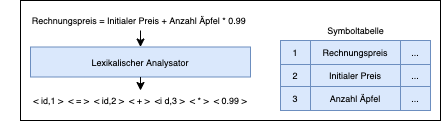
\includegraphics[width=\textwidth,keepaspectratio]{Images/Compiler/LexerResult.png}
 \caption[Exemplarische lexikalische Analyse]{Exemplarische lexikalische Analyse\protect\footcite{Ullmann2008}}
 \label{fig:LexerResult}
\end{figure}
\footnotetext{Abbildung in Anlehnung an Ullman et al. 2008, S.10.}

Der Lexer interagiert mit anderen Komponenten eines Compilers.  Klassischerweise wird der Lexer über den sogenannten Parser, welcher im nächsten Abschnitt eingeführt wird,  zur Übermittlung von Tokens aufgefordert.  Diese schematische Kommunikation wird in  Abbildung \ref{fig:LexerInteraktionen} dargestellt.  \footcite[Vgl.][S. 135]{Ullmann2008} 

\newpage
\begin{figure}[!ht]
 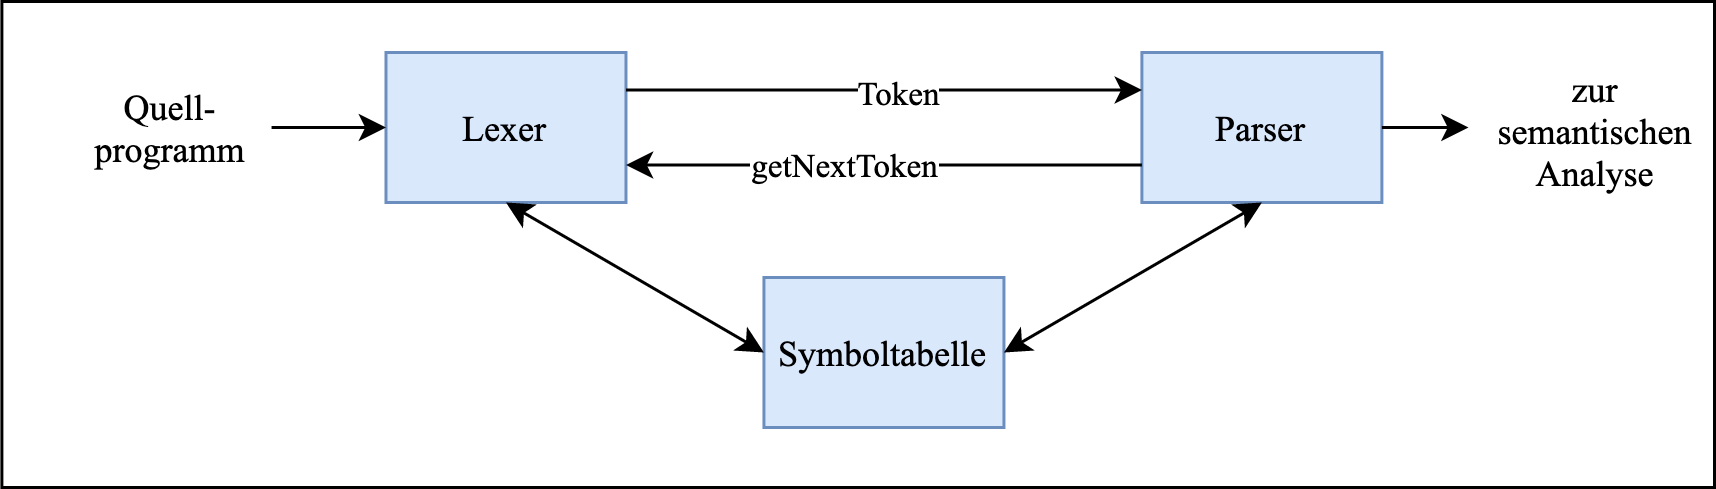
\includegraphics[width=\textwidth,keepaspectratio]{Images/Compiler/LexerParser.png}
 \caption[Interaktionen des Lexers]{Interaktionen des Lexers\protect\footcite{Ullmann2008}}
 \label{fig:LexerInteraktionen}
\end{figure}

Da der Lexer derjenige Teil des Compilers ist, der den Quelltext liest, kann er neben der Identifikation von Lexemen auch weitere Aufgaben übernehmen. \footnotetext{Abbildung in Anlehnung an Ullman et al. 2008, S.135.}So eignet er sich ideal zum Streichen von Kommentaren im Quelltext und zum Entfernen von Leerstellen,  wie Leerzeichen und Tabulatoren.  Zudem kann er gefundene Fehler den entsprechenden Zeilennummern zuordnen und dem Entwickler während der Kompilation so einen genauen Hinweis auf den Ort des Fehlers geben. \footcite[Vgl.][S. 135.]{Ullmann2008} 
Häufig werden Lexer daher in zwei kaskadierende Prozesse unterteilt, einen für das Löschen von Kommentaren und Zusammenfassung von Leerraumzeichen und einen für die eigentliche lexikalische Analyse.  \footcite[Vgl.][S. 136.]{Ullmann2008} 

\section{Syntaxanalyse}
In der zweiten Phase der Übersetzung, der Syntaxanalyse, werden durch den bereits erwähnten Parser, auch syntaktischer Analysator genannt, die vom Lexer ausgegebenen Tokens in eine baumartige Zwischendarstellung überführt, die die grammatikalische Struktur der Tokens zeigt.  Diese Darstellung wird basierend auf ihrem Aussehen häufig als Syntaxbaum bezeichnet.  Die Knoten im Syntaxbaum stehen für eine Operation und die Kindknoten für die Argumente dieser Operation.  Die Anordnung der Operationen stimmt mit üblichen arithmetischen Konventionen überein,  wie zum Beispiel dem Vorrang der Multiplikation vor Addition. \footcite[Vgl.][S. 9]{Ullmann2008} Abbildung \ref{fig:ParserResult} zeigt die Erstellung eines Syntaxbaumes aus den Tokens  der Abbildung \ref{fig:LexerResult}.  Anhand des Knotens \glq <id, 1>\grq{} ist jederzeit über die Symboltabelle ablesbar,  dass das Ergebnis der exemplarischen Rechnung an den Speicherort des Bezeichners Rechnungspreis abgelegt werden muss. \footcite[Vgl.][S. 9.]{Ullmann2008} 

\begin{figure}[!ht]
 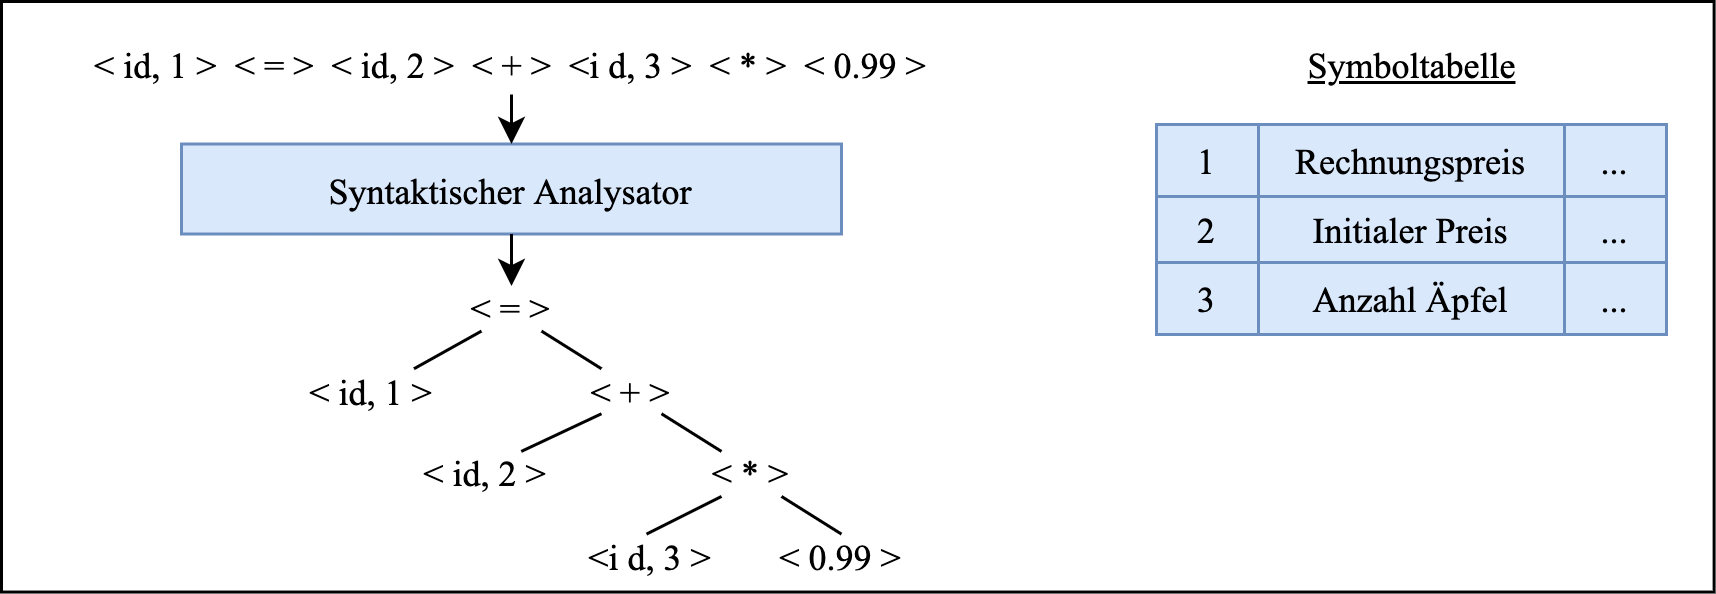
\includegraphics[width=\textwidth,keepaspectratio]{Images/Compiler/ParserResult.png}
 \caption[Exemplarischer Syntaxbaum]{Exemplarischer Syntaxbaum \protect\footcite{Ullmann2008} }
 \label{fig:ParserResult}
\end{figure}
\section{Semantische Analyse}

Bei der semantischen Analyse wird der Syntaxbaum  \footnotetext{Abbildung in Anlehnung an Ullman et al. 2008, S.10.}  als Aufgliederung der Programmstruktur,  zusammen mit den Informationen aus der Symboltabelle verwendet,  um das Quellprogramm auf semantische Konsistenz mit der Sprachdefinition zu überprüfen. \footcite[Vgl.][S. 157]{Wilhelm2012} Zudem werden hier Typinformationen gesammelt und zur späteren Verwendung im Syntaxbaum oder der Symboltabelle hinterlegt.  Auch findet eine Typüberprüfung statt die analysiert, ob jeder Operator die passenden Operanden hat.  So wird beispielsweise validiert,  ob ein Index eine Ganzzahl ist.  Es besteht die Möglichkeit, innerhalb des Baums Typkonvertierungen zu deponieren.  So wurde in dem bisherigen Beispiel die Anzahl Äpfel als Ganzzahl behandelt und wird für die Berechnung des Preises in Abbildung \ref{fig:Typ} zu einer Fließkommazahl konvertiert. \footcite[Vgl.][S. 9ff]{Ullmann2008}

\begin{figure}[!ht]
 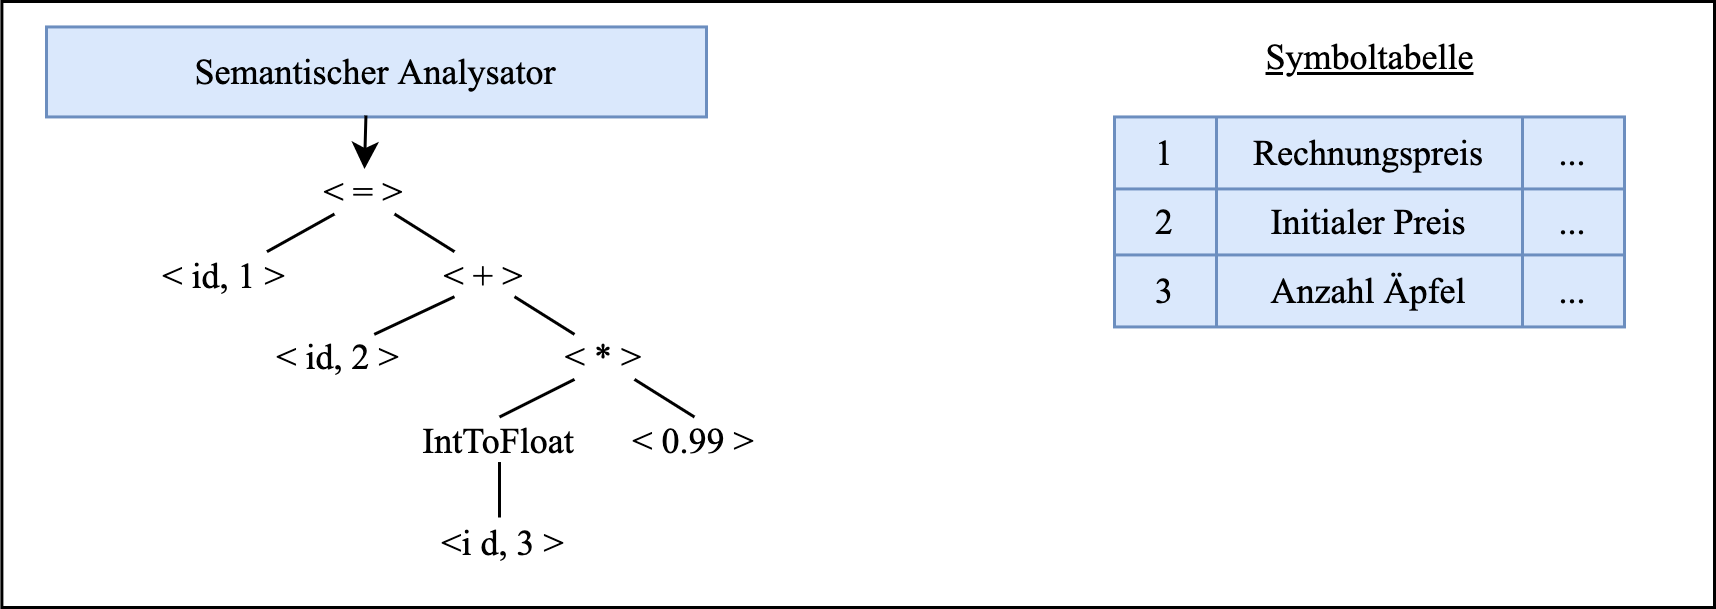
\includegraphics[width=\textwidth,keepaspectratio]{Images/Compiler/Type.png}
 \caption[Exemplarische Typüberprüfung]{Exemplarische Typüberprüfung \protect\footcite{Ullmann2008} }
 \label{fig:Typ}
\end{figure}
\footnotetext{Abbildung in Anlehnung an Ullman et al. 2008, S.10.} 
\section{Zwischencodeerzeugung}
Während der Übersetzung eines Programms  kann der Compiler mehrere Zwischendarstellungen in unterschiedlichsten Formen,  zum Beispiel die eines Syntaxbaums, erstellen.  
Nach der semantischen Analyse stellen viele Compiler eine maschinennahe Zwischendarstellung auf niedriger Abstraktionsebene her, die eigentlich für maschinenabhängige Aufgaben wie die Befehlsauswahl geeignet ist.  Eine Zwischendarstellung, die von Compiler zu Compiler in Auswahl oder Entwurf unterschiedlich ist,  kann entweder eine tatsächliche Sprache sein,  oder aus internen Datenstrukturen bestehen, die von den Phasen des Compilers gemeinsam verwendet werden. Auch wenn C eine Programmiersprache ist, wird sie häufig als eine Zwischenform verwendet, da sie flexibel ist, zu effizientem Maschinencode kompiliert werden kann und ihre Compiler weitgehend verfügbar sind.\footcite[Vgl.][S. 433]{Ullmann2008} Die variable Anzahl von Zwischendarstellungen bei der Kompilierung werden in Abbildung \ref{fig:Zwischendarstellung} skizziert.

\begin{figure}[!ht]
 
\includegraphics[width=\textwidth,keepaspectratio]{Images/Compiler/Zwischendarstellungen.png}
 \caption[Zwischendarstellungen]{Zwischendarstellungen \protect\footcite{Ullmann2008} }
 \label{fig:Zwischendarstellung}
\end{figure}

\section{Codeoptimierung}
In dieser Phase\footnotetext{Abbildung in Anlehnung an Ullman et al. 2008, S.433.}  wird der Code so optimiert, dass sich daraus ein besserer,  das heißt schnellerer oder ressourcenschonender Zielcode ergibt.  Der Umfang der Codeoptimierung schwankt dabei von Compiler zu Compiler erheblich.  \footcite[Vgl.][S. 11f]{Ullmann2008} 
Die Codeoptimierung, die ein Compiler vornimmt, ist im Laufe der Zeit wichtiger und umfangreicher geworden. Grund für die zunehmenden Anforderungen sind die immer komplexeren Prozessorarchitekturen, die mehr Gelegenheiten bieten, die Ausführung des  Codes zu verbessern. Die gestiegene Bedeutung ergibt sich beispielsweise aus der steigenden Anzahl an Kernen in modernen Computern und der Möglichkeit, Programme parallel auszuführen.\footcite[Vgl.][S. 20]{Ullmann2008}

\section{Codeerzeugung}
Die Überführung aus der Zwischendarstellung in die Zielsprache nennt man Codeerzeugung.  Hierbei muss die semantische Bedeutung des Quellprogramms erhalten und hochwertig dargestellt sein. Die größte Herausforderung ergibt sich aus der nicht komplett mathematischen Berechenbarkeit aller Prozesse bei der Überführung. Ein Beispiel wäre die Vergabe von Registern,  die nicht effizient berechenbar sind.  In der Praxis müssen heuristische Techniken ausreichen- die guten, aber nicht unbedingt optimalen Code liefern.  Die Codeoptimierungs- und  Codeerzeugungsphasen können mehrfach durchlaufen werden,  bevor das Zielprogramm finalisiert ist. \footcite[Vgl.][S. 618f]{Ullmann2008}

\section{Der .NET Compiler Roslyn}
Für die Arbeit mit der Programmiersprache \Csharp{} steht mit Roslyn ein Compiler zur Verfügung, der sich aus modularen Bibliotheken zusammensetzt.  Durch die Referenzierung dieser Bibliotheken können Programme auf den Funktionsumfang von Roslyn zugreifen.  So ist es möglich, den Compiler zu verwenden, ohne das Ziel zu haben, die Programmiersprache \Csharp{} in plattformnahen Code zu übersetzen.  Dabei stehen die Bibliotheken über den Packetmanager Nuget für die Einbindung in eigene Projekte zur Verfügung.  Um diese Funktionalität zu gewährleisten,  unterteilt Rosyln die Übersetzung in mehrere Phasen,  welche wiederum einige der in diesem Kapitel beschriebenen Phasen zusammenfassen. Die erste Phase ist die Erstellung des Syntaxbaums, die zweite Phase ist die semantische Analyse gefolgt von der letzten Phase der Ausgabe der so genannten Intermediate Language als Zielsprache. \footcite[Vgl.][S. 1017]{Albahari2020}



